\documentclass{article}

%%%%%%%%%%%%%%%%%%%%%%%%
% All the packages                                              %
%%%%%%%%%%%%%%%%%%%%%%%%

\usepackage{amsmath} % Required for many math properties. AMS stands for American Mathematical Society.
\usepackage{amssymb} %Required for using many math symbols.
\usepackage{geometry} % Required for adjusting page dimensions.
\usepackage[T1]{fontenc} % Defines how ASCII is mapped
\usepackage[utf8]{inputenc} % Required for inputting international characters.
\usepackage[none]{hyphenat} % Removes automatic hyphenation (a personal pet peeve of Sam).
\usepackage{graphicx} % Required to inlcude graphics.
\usepackage{hyperref} % Required to include URLs.
\usepackage{xcolor} % Required to turn URLs the correct colors.
\usepackage{listings} % Required to display code.
\usepackage{tikz} % Required to 
\usepackage{float} % Helpful for table/photo positioning
\usepackage{wrapfig} % Helpful for photo captioning
\usepackage{multicol} % Easily make nice columns with greater flexibility than LaTeX \twocolumn
\usepackage{enumitem} % Make fancy enumerate/itemize environments
\usepackage[rm, light]{roboto} % This makes roboto slab light (AKA, the font Google uses) the main document font
\usepackage{titlesec} % Allows section spacing manipulations
\usepackage{bm} % Allows mathmode characters to be bolded
\usepackage{grffile} % Lets spaces be included in image filenames
\usepackage{tikzsymbols} % More symbols in tikz
\usepackage[most]{tcolorbox} % Allows for color 
\usepackage{imakeidx} % Creates an index
\usepackage[edges]{forest} % Allows us to create graphs/forests
\usepackage{nameref} % Helps with references
\usepackage{stringstrings} % String and variable manipulation
\usepackage{lipsum} % Dummy text


%%%%%%%%%%%%%%%%%%%%%%%%%
% Book Style Page Numbers
%%%%%%%%%%%%%%%%%%%%%%%%%

%\usepackage{etoolbox} 
%\usepackage{fancyhdr}
%\pagestyle{fancy}
%\fancyhead[RO]{\slshape \rightmark}
%\fancyhead[LE]{\slshape \leftmark}
%\fancyhead[LO,RE]{\thepage}
%\renewcommand{\headrulewidth}{0pt}
%\renewcommand{\footrulewidth}{0pt}
%\cfoot{} % get rid of the page number 
%\patchcmd{\chapter}{\thispagestyle{plain}}{\thispagestyle{fancy}}{}{}

%%%%%%%%%%%%%%%%%%%%%%%%
% Start Indexing Document                                              %
%%%%%%%%%%%%%%%%%%%%%%%%

%\makeindex

%%%%%%%%%%%%%%%%%%%%%%%%
% Set document colorscheme                                             %
%%%%%%%%%%%%%%%%%%%%%%%%


% Primary Color
\definecolor{blue0}{HTML}{133667}
\definecolor{blue1}{HTML}{3C5F8F}
\definecolor{blue2}{HTML}{23497D}
\definecolor{blue3}{HTML}{06254F}
\definecolor{blue4}{HTML}{021733}
% Main Secondary color (1)
\definecolor{red0}{HTML}{9D1811}
\definecolor{red1}{HTML}{D95750}
\definecolor{red2}{HTML}{BE2F28}
\definecolor{red3}{HTML}{780600}
\definecolor{red4}{HTML}{4E0400}
% Main Secondary color (2)
\definecolor{green0}{HTML}{0D791A}	
\definecolor{green1}{HTML}{3EA94B}
\definecolor{green2}{HTML}{1F932D}
\definecolor{green3}{HTML}{005D0B}
\definecolor{green4}{HTML}{003C07}
% Main Complement color
\definecolor{yellow0}{HTML}{9D6811}	
\definecolor{yellow1}{HTML}{D9A650}
\definecolor{yellow2}{HTML}{BE8628}

%%%%%%%%%%%%%%%%%%%%%%%%
% Define color/formatting for chapter and section names       
%%%%%%%%%%%%%%%%%%%%%%%%

\titleformat{\chapter}
{\color{blue0}\normalfont\huge\bfseries}
{\color{blue0}\thechapter}{1em}{}


\titleformat{\section}
{\color{blue2}\normalfont\huge\bfseries}
{\color{blue2}\thesection}{1em}{}

%%%%%%%%%%%%%%%%%%%%%%%%
% Applies coloring to textbf and textit; note that roboto does not allow italics. %
%
% Also colors list bullet points.
%%%%%%%%%%%%%%%%%%%%%%%%

\let\oldtextbf\textbf
\renewcommand{\textbf}[1]{\textcolor{blue1}{\oldtextbf{#1}}}

\let\oldtextit\textit
\renewcommand{\textit}[1]{\textcolor{red0}{\oldtextit{#1}}}

%%%%%%%%%%%%%%%%%%%%%%%%
% Auto bold and add any word with the command \ibf{Keyword} to the index.  %
%%%%%%%%%%%%%%%%%%%%%%%%

\newcommand{\ibf}[1]{\index{\capitalizetitle{#1}}\textbf{\mbox{#1}}}




%%%%%%%%%%%%%%%%%%%%%%%%
% Frame and organize images  %
%%%%%%%%%%%%%%%%%%%%%%%%


\setlength{\fboxsep}{0.2em}%
\setlength{\fboxrule}{0.25em}%

\let\oldincludegraphics\includegraphics

\renewcommand{\includegraphics}[2][]{\fcolorbox{blue0}{white}{\oldincludegraphics[#1]{#2}}}

%%%%%%%%%%%%%%%%%%%%%%%%
% Make custom changes to lists  %
%%%%%%%%%%%%%%%%%%%%%%%%


%\setlist[itemize]{leftmargin=0pt}

\renewcommand{\labelitemi}{\textcolor{red0}{$\bullet$}}


%%%%%%%%%%%%%%%%%%%%%%%%
% Set up normal hyperlink colors, colorscheme be damned.
%%%%%%%%%%%%%%%%%%%%%%%%
\hypersetup{
	colorlinks,
	linkcolor={black!50!black},
	citecolor={blue!50!black},
	urlcolor={black!80!black}
}

%%%%%%%%%%%%%%%%%%%%%%%%
% Set up page dimensions.
%%%%%%%%%%%%%%%%%%%%%%%%
\geometry{
	papersize={8.5in,11in}, % 8.5 x 11 paper.
	margin=1in
}
%%%%%%%%%%%%%%%%%%%%%%%%
% Set up code display settings
%%%%%%%%%%%%%%%%%%%%%%%%
\lstset{
	frame = single, % Box the code
	numbers=left % Show line numbers
}
%%%%%%%%%%%%%%%%%%%%%%%%
% Set up line and paragraph spacing
%%%%%%%%%%%%%%%%%%%%%%%%
\setlength{\parindent}{0em} % Sets paragraph indentation
\setlength{\parskip}{0.75em} % Sets paragraph spacing
\linespread{1.0} % Sets line spacing
\renewcommand{\arraystretch}{1.5}

%%%%%%%%%%%%%%%%%%%%%%%%
% Have footnotes use symbols, not numbers.
%%%%%%%%%%%%%%%%%%%%%%%%
\renewcommand{\thefootnote}{\alph{footnote}}


%%%%%%%%%%%%%%%%%%%%%%%%
% When using Lorium Ipsum dummy text, only print out 1 paragraph at a time by default
%%%%%%%%%%%%%%%%%%%%%%%%
%\setlipsumdefault{1}


%%%%%%%%%%%%%%%%%%%%%%%%
% All your favorite math shortcuts
%%%%%%%%%%%%%%%%%%%%%%%%


\newcommand{\C}{\mathbb{C}}
\newcommand{\R}{\mathbb{R}}
\newcommand{\I}{\mathbb{I}}
\newcommand{\Q}{\mathbb{Q}}
\newcommand{\N}{\mathbb{N}}
\newcommand{\Z}{\mathbb{Z}}
\newcommand{\e}{\epsilon}
\renewcommand{\d}{\delta}
\newcommand{\D}{\Delta}
\renewcommand{\a}{\alpha}
\renewcommand{\b}{\beta}
\renewcommand{\l}{\lambda}
\renewcommand{\t}{\theta}
\renewcommand{\P}{\mathcal{P}}
\newcommand{\G}{\mathcal{G}}
\newcommand{\DD}{\mathbb{D}}
\newcommand{\nk}[2]{\binom{#1}{#2}}
\newcommand{\nkf}[2]{\frac{(#1)!}{(#2)!\cdot ((#1)-(#2))!}}
\newcommand{\NOT}{\neg}
\newcommand{\AND}{\wedge}
\newcommand{\OR}{\vee}

\newcommand{\ceil}[1]{\lceil #1 \rceil}
\newcommand{\floor}[1]{\lfloor #1 \rfloor}

\newcommand{\bvec}[1]{\begin{bmatrix}#1\end{bmatrix}}
\newcommand{\pvec}[1]{\begin{pmatrix}#1\end{pmatrix}}


\title{Data, Decisions, and AI/ML Discoveries: Lab B}
\date{\textbf{This is an optional lab, for which no credit will be given.}}

\author{Dr. Sam Schwartz}

\begin{document}
	
	\maketitle

\section{Objectives}
On completing this project, you will be able to:

\begin{enumerate}
	\item Load data from a text file
	\item Visualize data with matplotlib
	\item Create a k nearest neighbors model with Python
	\item Create a decision tree with Python
\end{enumerate}

\section{Case Study}





\section{The Project}

\begin{center}
	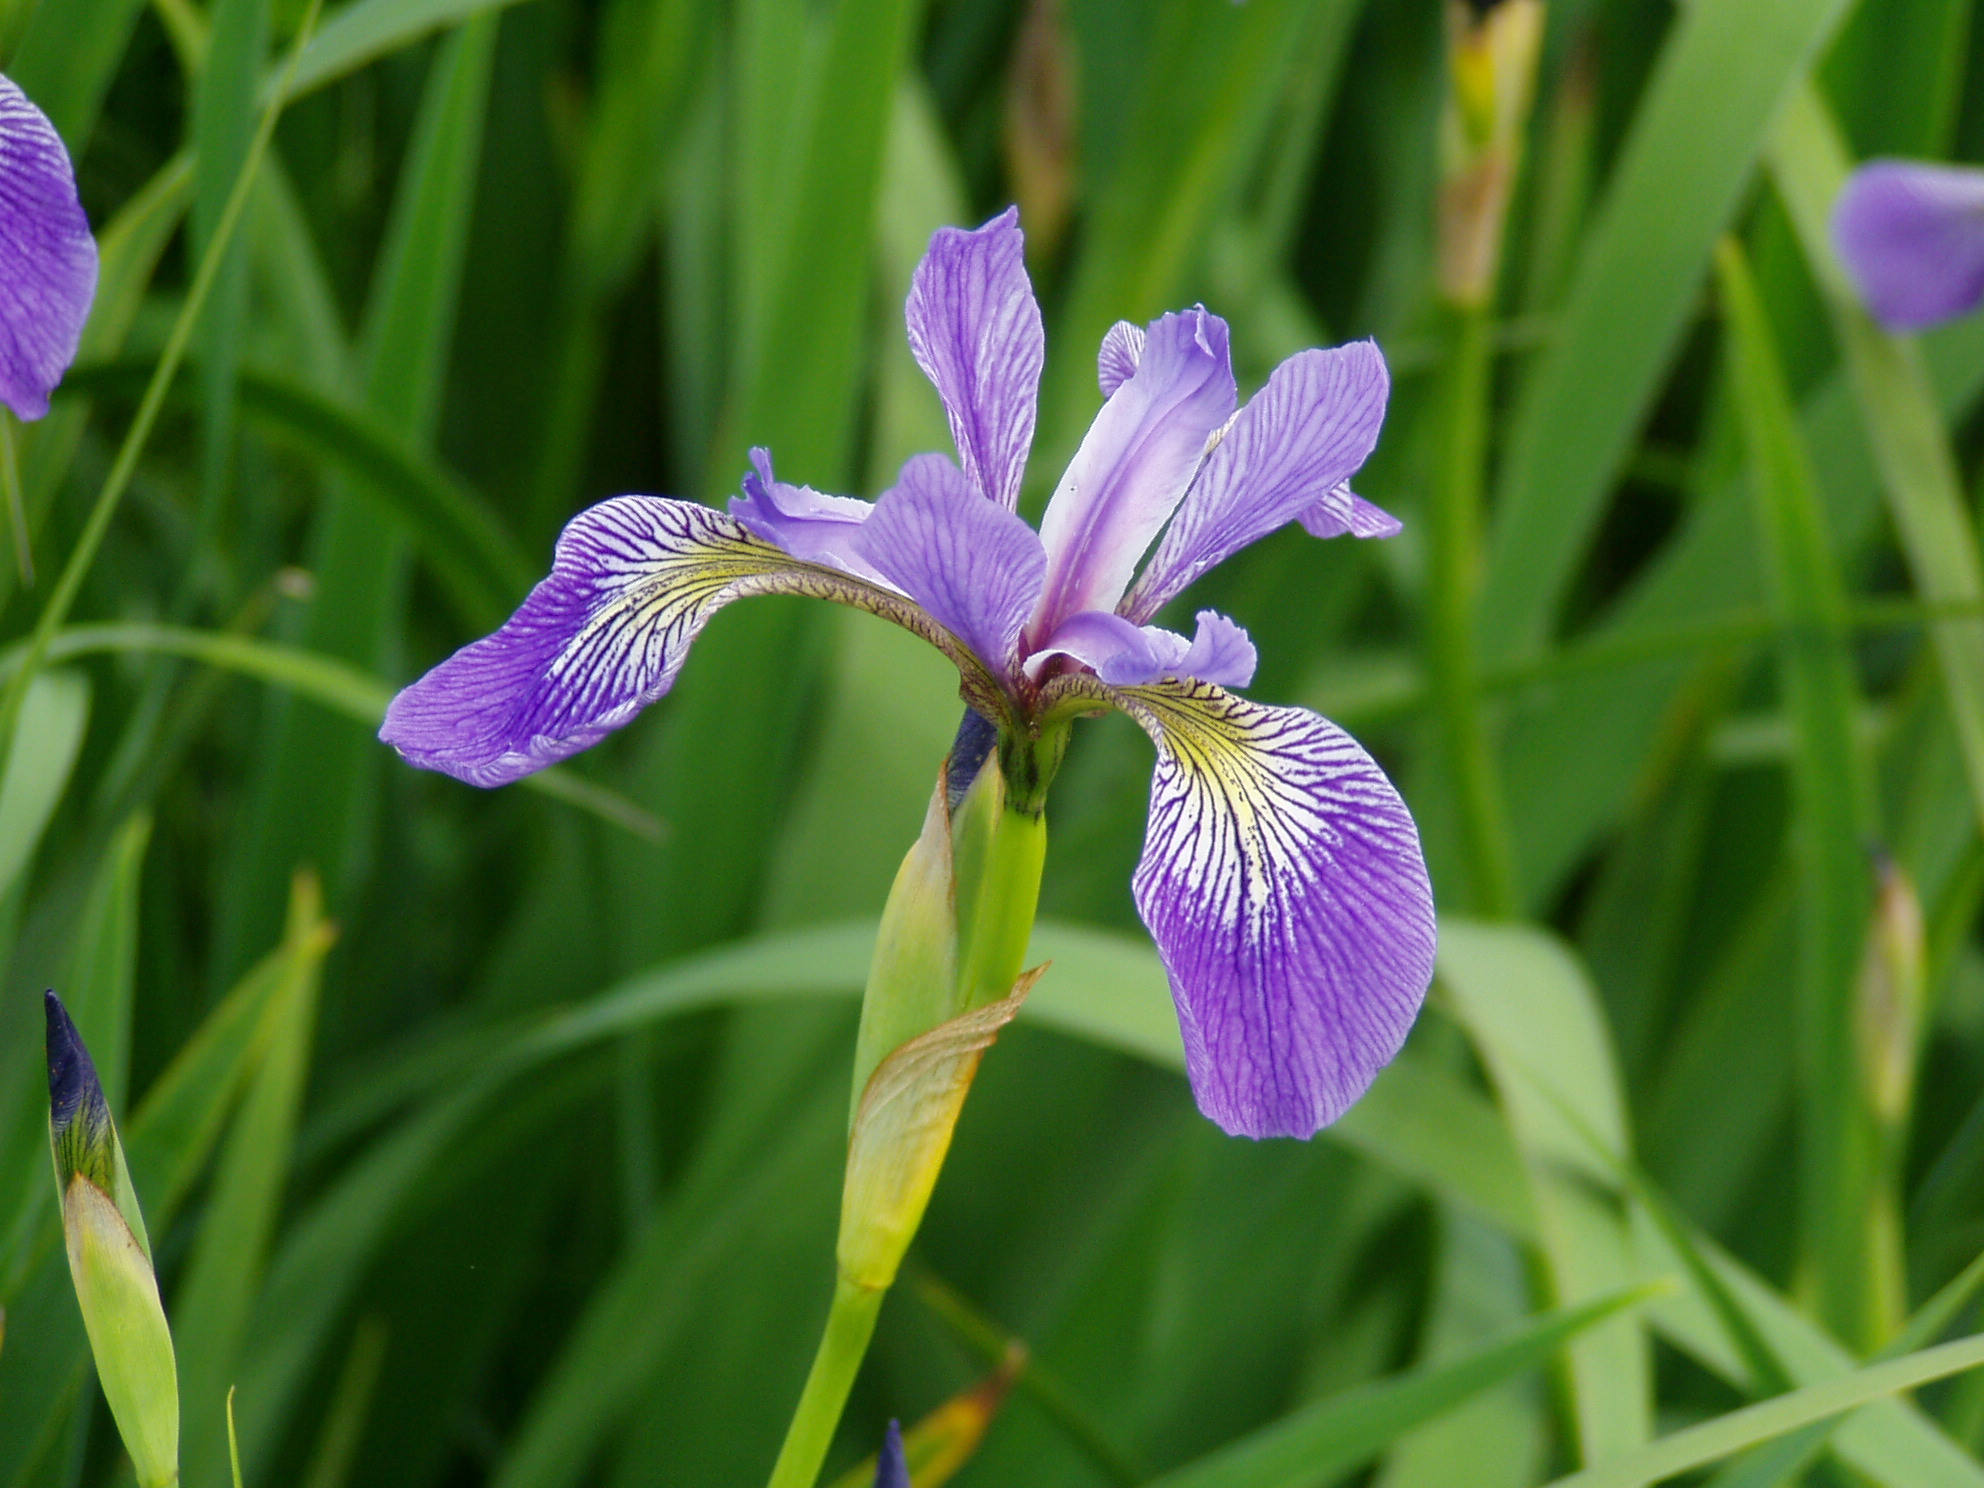
\includegraphics[width=0.5\linewidth]{iris.jpg}
	
	An example of an iris in bloom.
\end{center}

An iris is a kind of flower. You are given 150 rows of data. Each row represents information about a particular iris flower someone went and looked at.

The data is stored in a file called \texttt{iris\_data.csv}. The first row is the header.

Recorded in the first column is the species of the flower. It is encoded here as a number: 1, 2, or 3.

Recorded in the second column is the average area of the flower's sepals in cm$^2$.

Recorded in the third column is the average area of the flower's petals in cm$^2$.


Our goal is, given sepal area and petal area, to predict if a new flower's species is 1, 2, or 3.

We will do so in a visual way: by plotting the decision boundary of a classifier.\footnote{We will not be doing any validation on our classifier for this project. All data is to be used as training data.}



\subsection{Deliverables}

A Python program which:

\begin{enumerate}
	\item Uses the sci-kit learn framework to classify data using at least two classifiers.
	\item Plots the decision areas for each classifier.
	\item Includes a scatter plot of the training data overlaying the decision area. 
	\item Displays these plots on the screen.
\end{enumerate}

%You should upload a single .py file to Canvas for assessment. 

\section{Ideal Output}

Figures analogous to these:

\begin{center}
	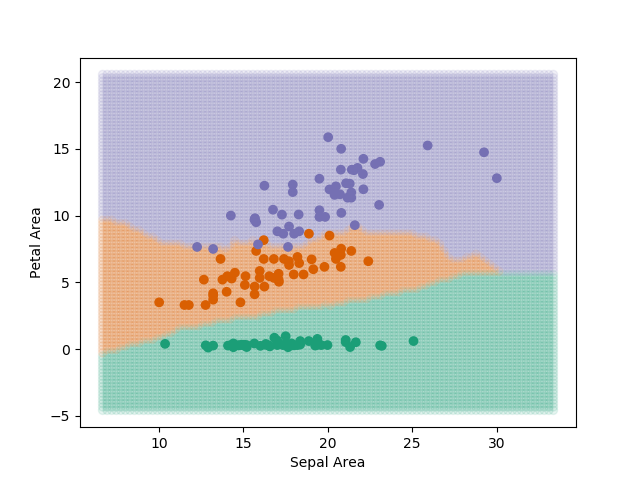
\includegraphics[width=0.75\linewidth]{Figure1.png}
	
	Decision areas of a nearest neighbors classifier. Training data is overlayed.
\end{center}

\begin{center}
	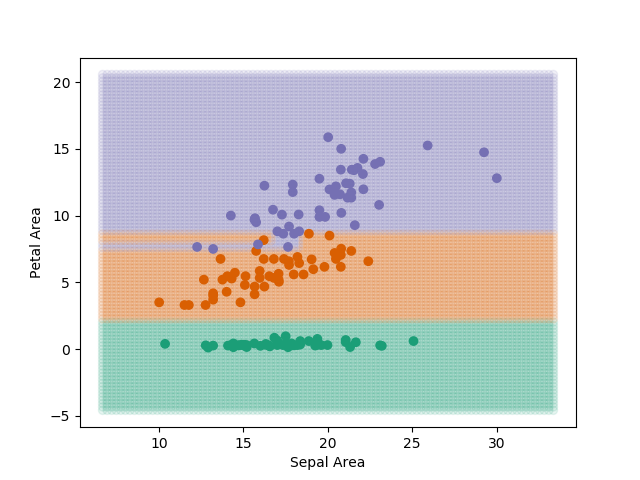
\includegraphics[width=0.75\linewidth]{Figure2.png}
	
	Decision areas of a single decision tree. Training data is overlayed.
\end{center}

%\clearpage
%\section{Grading Rubric}
%
%\subsection{Validity}
%The Author's code plotted a decision area for all classifiers\dotfill 4\quad3\quad2\quad1\quad0\\
%The Author's code plotted the training data overlaying the decision boundary for all classifiers  \dotfill  4\quad3\quad2\quad1\quad0\\
%The plots were displayed on the screen \dotfill  2\quad1\quad0\\
%
%\textbf{Validity Total: }\dotfill \qquad\qquad\qquad of 10.\\
%
%\subsection{Readability}
%
%Score provided by the auto-grader for readability: \dotfill 10\quad9\quad8\quad7\quad6\quad5\quad4\quad3\quad2\quad1\quad0
%
%\subsection{Fluency}
%
%(Obj 1.) Author's code used the sk-learn framework.\dotfill 2\quad1\quad0\\
%(Obj 2.) Author's code utilized two different classifiers.\dotfill 2\quad1\quad0\\
%(Obj 3.) Author's code predicted the class for new points.\dotfill 2\quad1\quad0\\
%(Obj 4.) Author's code efficiently used an external module for plotting.\dotfill 2\quad1\quad0\\
%
%Author's code was elegant:  \dotfill 2\quad1\quad0
%
%
%\vspace{1in}
%
%
%
%
%\textbf{Fluency Total: }\dotfill \qquad\qquad\qquad of 10.\\
%
%\textbf{Project Total: }\dotfill \qquad\qquad\qquad of 25.


\end{document}
